\begin{frame}{Etablering af levende hegn og linieformede markopdelinger}

\small

\begin{columns}[T]

\begin{column}{0.58\textwidth}

\textbf{Regler for etablering af levende hegn og linieformede markopdelinger:}

\begin{itemize}[]
\item Min. 2 m bred
\item Anlægges langs grøfter, diger, veje mm.
\item Ved mere end tre rækker: lysåbning hver 50. meter
\end{itemize}

\vspace{0.4em}

\textbf{Gavner arter:}

\footnotesize
Fasan, agerhøne, markhare, rådyr, dådyr, rødrygget tornskade, gul vipstjert, 
pirol, gulspurv, blåmejse, musvit, sortmejse, grønsisken, stillits, rødhals, 
nattergal, hærfugl, flagermus, pindsvin, lækat, egern, musvåge, spurvehøg, 
tårnfalk, rørhøg

\end{column}

\begin{column}{0.40\textwidth}
\centering
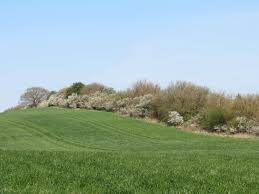
\includegraphics[width=\textwidth]{Billeder/Vildtforvaltning/biotopplantiltag/levendehegn.jpeg}
\end{column}

\end{columns}

\end{frame}